\documentclass[tikz, border=2pt]{standalone}

\usepackage{amsmath,amssymb}
\usepackage{pgfplots}
\pgfplotsset{compat=1.18}
\usepgfplotslibrary{groupplots}
\usepackage{xcolor}

\definecolor{utnblue}{RGB}{0, 51, 102}
\definecolor{utnred}{RGB}{204, 0, 0}

\begin{document}
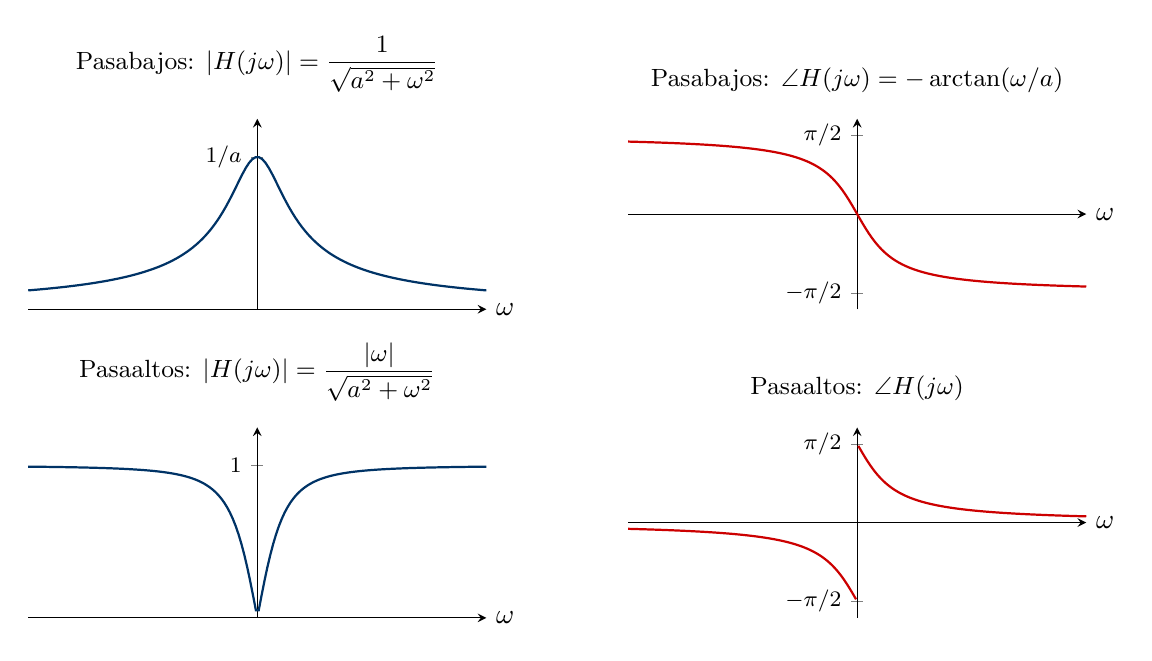
\begin{tikzpicture}

\begin{groupplot}[
    group style={group size=2 by 2, horizontal sep=1.8cm, vertical sep=1.5cm},
    width=7.4cm, height=4.0cm,
    axis lines=middle,
    enlargelimits=false,
    tick label style={font=\footnotesize},
    label style={font=\small},
    title style={font=\small},
    every axis x label/.style={at={(ticklabel* cs:1)}, anchor=west},
]

% --- Pasabajos: modulo ---
\nextgroupplot[
    title={Pasabajos: $|H(j\omega)| = \dfrac{1}{\sqrt{a^2+\omega^2}}$},
    xlabel={$\omega$}, xmin=-8, xmax=8, ymin=0, ymax=1.25,
    xtick=\empty, ytick={1}, yticklabels={$1/a$},
]
\addplot[utnblue, thick, samples=140, domain=-8:8] {1/sqrt(1+x*x)};

% --- Pasabajos: fase ---
\nextgroupplot[
    title={Pasabajos: $\angle H(j\omega) = -\arctan(\omega/a)$},
    xlabel={$\omega$}, xmin=-8, xmax=8, ymin=-1.9, ymax=1.9,
    xtick=\empty, ytick={-1.5708,1.5708}, yticklabels={$-\pi/2$,$\pi/2$},
]
\addplot[utnred, thick, samples=140, domain=-8:8] {-atan(x)*pi/180};

% --- Pasaaltos: modulo ---
\nextgroupplot[
    title={Pasaaltos: $|H(j\omega)| = \dfrac{|\omega|}{\sqrt{a^2+\omega^2}}$},
    xlabel={$\omega$}, xmin=-8, xmax=8, ymin=0, ymax=1.25,
    xtick=\empty, ytick={1}, yticklabels={$1$},
]
\addplot[utnblue, thick, samples=160, domain=-8:8] {abs(x)/sqrt(1+x*x)};

% --- Pasaaltos: fase ---
\nextgroupplot[
    title={Pasaaltos: $\angle H(j\omega)$},
    xlabel={$\omega$}, xmin=-8, xmax=8, ymin=-1.9, ymax=1.9,
    xtick=\empty, ytick={-1.5708,1.5708}, yticklabels={$-\pi/2$,$\pi/2$},
]
\addplot[utnred, thick, samples=120, domain=0.04:8] {pi/2 - atan(x)*pi/180};
\addplot[utnred, thick, samples=120, domain=-8:-0.04] {-pi/2 - atan(x)*pi/180};

\end{groupplot}

\end{tikzpicture}
\end{document}
